\documentclass[tikz,border=10pt]{standalone}
\usepackage{amsmath}
\usepackage{amssymb}
\usepackage{tikz}
\usetikzlibrary{arrows.meta,calc}

\definecolor{figazul}{RGB}{2,132,199}
\definecolor{figrojo}{RGB}{220,38,38}
\definecolor{figverde}{RGB}{22,163,74}

\begin{document}
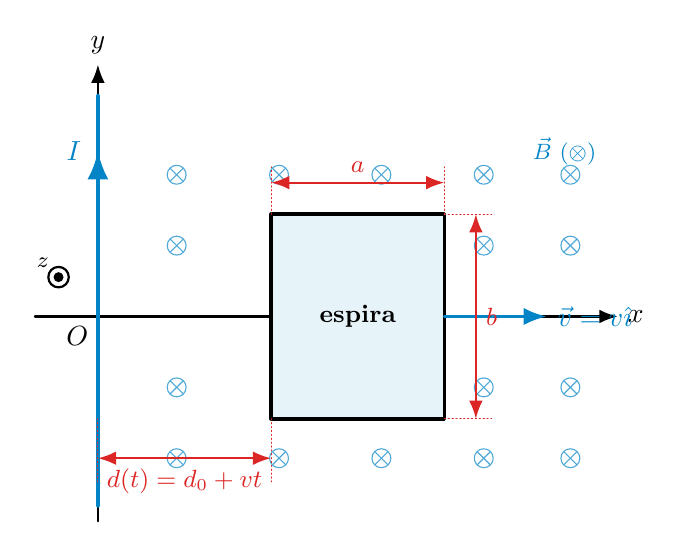
\begin{tikzpicture}[>=Latex, line cap=round, line join=round]
  % Ejes de coordenadas
  \draw[->, thick] (-0.8, 0) -- (6.6, 0) node[right] {$x$};
  \draw[->, thick] (0, -2.6) -- (0, 3.2) node[above] {$y$};
  \node[below left] at (0,0) {$O$};

  % Eje z saliente cerca del origen
  \draw[thick] (-0.5, 0.5) circle (0.13);
  \fill (-0.5, 0.5) circle (1.8pt);
  \node[above left, font=\footnotesize] at (-0.5, 0.5) {$z$};

  % Cable infinito sobre el eje y con corriente I hacia +y
  \draw[ultra thick, color=figazul] (0, -2.4) -- (0, 2.8);
  \draw[->, ultra thick, color=figazul] (0, 1.2) -- (0, 2.1) node[left=2pt, color=figazul] {$I$};

  % Grilla regular de campo magnético entrante \vec{B} (\otimes) en x > 0
  \foreach \gx in {1.0, 2.3, 3.6, 4.9, 6.0} {
    \foreach \gy in {-1.8, -0.9, 0.9, 1.8} {
      \draw[thin, color=figazul!70] (\gx, \gy) circle (0.12);
      \draw[thin, color=figazul!70] (\gx-0.08, \gy-0.08) -- (\gx+0.08, \gy+0.08);
      \draw[thin, color=figazul!70] (\gx-0.08, \gy+0.08) -- (\gx+0.08, \gy-0.08);
    }
  }
  \node[above right, font=\footnotesize, color=figazul] at (5.4, 1.8) {$\vec{B}$ ($\otimes$)};

  % Espira rectangular de lados a x b
  % x va desde d(t) = 2.2 hasta d(t)+a = 4.4
  % y va desde -1.3 hasta +1.3 (b = 2.6)
  \def\dt{2.2}
  \def\a{2.2}
  \def\b{2.6}
  \def\ybot{-1.3}
  \def\ytop{1.3}

  \draw[very thick, fill=figazul!10] (\dt, \ybot) rectangle (\dt+\a, \ytop);
  \node[font=\small\bfseries] at (\dt + 0.5*\a, 0) {espira};

  % Vector velocidad v hacia +x
  \draw[->, very thick, color=figazul] (\dt+\a, 0) -- (\dt+\a+1.3, 0) node[right, color=figazul] {$\vec{v} = v\hat{\imath}$};

  % Cotas en rojo
  % Cota d(t) desde x = 0 hasta borde izquierdo
  \draw[<->, thick, color=figrojo] (0, -1.8) -- (\dt, -1.8) node[midway, below, color=figrojo, font=\small] {$d(t) = d_0 + vt$};
  \draw[densely dotted, thin, color=figrojo] (\dt, \ybot) -- (\dt, -2.1);
  \draw[densely dotted, thin, color=figrojo] (0, \ybot) -- (0, -2.1);

  % Cota a (ancho de la espira)
  \draw[<->, thick, color=figrojo] (\dt, \ytop+0.4) -- (\dt+\a, \ytop+0.4) node[midway, above, color=figrojo, font=\small] {$a$};
  \draw[densely dotted, thin, color=figrojo] (\dt, \ytop) -- (\dt, \ytop+0.6);
  \draw[densely dotted, thin, color=figrojo] (\dt+\a, \ytop) -- (\dt+\a, \ytop+0.6);

  % Cota b (altura de la espira)
  \draw[<->, thick, color=figrojo] (\dt+\a+0.4, \ybot) -- (\dt+\a+0.4, \ytop) node[midway, right, color=figrojo, font=\small] {$b$};
  \draw[densely dotted, thin, color=figrojo] (\dt+\a, \ybot) -- (\dt+\a+0.6, \ybot);
  \draw[densely dotted, thin, color=figrojo] (\dt+\a, \ytop) -- (\dt+\a+0.6, \ytop);

\end{tikzpicture}
\end{document}
